% This file was created with tikzplotlib v0.9.16.
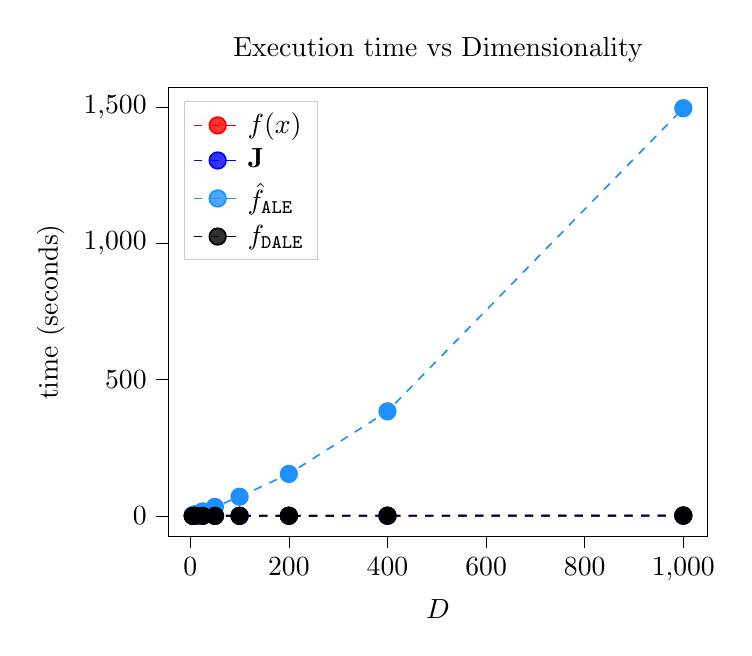
\begin{tikzpicture}

\definecolor{color0}{rgb}{0.117647058823529,0.564705882352941,1}

\begin{axis}[
legend cell align={left},
legend style={
  fill opacity=0.8,
  draw opacity=1,
  text opacity=1,
  at={(0.03,0.97)},
  anchor=north west,
  draw=white!80!black
},
tick align=outside,
tick pos=left,
title={Execution time vs Dimensionality},
x grid style={white!69.0196078431373!black},
xlabel={\(\displaystyle D\)},
xmin=-44.75, xmax=1049.75,
xtick style={color=black},
y grid style={white!69.0196078431373!black},
ylabel={time (seconds)},
ymin=-74.5375274447479, ymax=1569.39754059975,
ytick style={color=black}
]
\addplot [semithick, red, dashed, mark=*, mark size=3, mark options={solid}]
table {%
5 0.277210694999667
10 0.281487796000874
25 0.284969493000972
50 0.316298918998655
100 0.305420158001652
200 0.372751692000747
400 0.439941012999043
1000 0.595708296998055
};
\addlegendentry{$f(x)$}
\addplot [semithick, blue, dashed, mark=*, mark size=3, mark options={solid}]
table {%
5 0.186793830001989
10 0.187544139000238
25 0.19816158300091
50 0.205550107002637
100 0.205516074001935
200 0.235798017998604
400 0.259789005001949
1000 0.424904576000699
};
\addlegendentry{$\mathbf{J}$}
\addplot [semithick, color0, dashed, mark=*, mark size=3, mark options={solid}]
table {%
5 2.91359372999796
10 6.11244208399876
25 16.2270338710005
50 32.7731953399998
100 70.2450085599994
200 153.828656939997
400 383.318796881998
1000 1494.673219325
};
\addlegendentry{$\hat{f}_{\mathtt{ALE}}$}
\addplot [semithick, black, dashed, mark=*, mark size=3, mark options={solid}]
table {%
5 0.19148760600001
10 0.206710942999052
25 0.230522152000049
50 0.279659739000635
100 0.34547448900048
200 0.591088396999112
400 0.816774448001524
1000 1.8221750010016
};
\addlegendentry{$f_{\mathtt{DALE}}$}
\end{axis}

\end{tikzpicture}
